\documentclass[a4paper, 12pt, final, garamond]{book}
\usepackage{cours-preambule}

\titleformat{\subsection}{}{\arabic{subsection})}{.5em}{}{}
\titleformat{\subsubsection}{}{\arabic{subsection}) \alph{subsubsection} --}{.5em}
{}{}

\raggedbottom

\makeatletter
\renewcommand{\@chapapp}{\'Electrocin\'etique -- chapitre}
\makeatother

\begin{document}
\setcounter{chapter}{1}

\chapter{Correction du TD}

\section{Circuit simple}\label{ch2:ex1}
\begin{center}
    \begin{NCdefi}[width=.5\linewidth]{Données}
        Générateur \underline{réel} $(E,r)$ de tension~: \smallbreak
        \begin{center}
            \includegraphics{circ_simple-a}
        \end{center}
    \end{NCdefi}
\end{center}

\subsection{}
\begin{tcbraster}[raster columns=3, raster equal height=rows]
    \begin{NCprop}{Résultat attendu}
        On demande un schéma \underline{normalisé}, autrement dit avec les
        conventions de schémas \textit{européennes}.
    \end{NCprop}
    \begin{NCrapp}{Outils}
        Générateur~:
        \includegraphics{circ_simple-b}
        \smallbreak
        Résistance~:\vspace{12pt}
        \includegraphics{circ_simple-c}
    \end{NCrapp}
    \begin{NCcexe}{Application}
        On obtient~: \smallbreak
        \includegraphics{circ_simple-d}
    \end{NCcexe}
\end{tcbraster}

\subsection{}
\begin{tcbraster}[raster columns=2, raster equal height=rows]
    \begin{NCrapp}{Outils}
        Générateur convention générateur~: \smallbreak
        \vspace{-12pt}
        \begin{center}
            \includegraphics{circ_simple-e}
        \end{center}
        Résistance convention récepteur~: \smallbreak
        \vspace{-12pt}
        \begin{center}
            \includegraphics{circ_simple-f}
        \end{center}
    \end{NCrapp}
    \begin{NCexem}{Application}
        \begin{center}
            \includegraphics{circ_simple-g}
        \end{center}
    \end{NCexem}
\end{tcbraster}

\subsection{}
\begin{tcbraster}[raster columns=5, raster equal height=rows]
    \begin{NCprop}[raster multicolumn=2]{Résultat attendu}
        À partir d'un circuit où on considère $E$, $r$ et $R$ comme des
        grandeurs connues, on cherche l'intensité $I$ qui parcourt la maille que
        l'on vient de tracer.
    \end{NCprop}
    \begin{NCrema}[raster multicolumn=3]{Remarque}
        Il y a deux outils qui seront utiles pour déterminer des grandeurs dans
        des circuits~: la \textbf{loi des mailles} et la \textbf{loi des nœuds}.
        À cela se rajoute la \textbf{loi d'Ohm} qui relie tension et intensité
        dans une résistance. Ces notions seront vues dans le chapitre suivant et
        donc décrites ultérieurement, on va ici utiliser la composition des
        tensions.
    \end{NCrema}
\end{tcbraster}
\begin{tcbraster}[raster columns=3, raster equal height=rows]
    \begin{NCrapp}{Outil}
        En nommant des points d'intérêt du circuit, ce qui est souvent
        conseillé, on va pouvoir utiliser la composition $U_\mathrm{AC} =
        U_\mathrm{AB} + U_\mathrm{BC}$ en respectant le sens des tensions pour
        obtenir une information supplémentaire sur le circuit. \smallbreak
        On rappelle que deux points sur un fil sont au même potentiel, et on
        peut donc les nommer de la même manière.
    \end{NCrapp}
    \begin{NCexem}[raster multicolumn=2, sidebyside]{Application}
        \tcbsubtitle[before skip=\baselineskip,
        colback = darkgray!50!black,
        colframe = darkgray!50!black]{Schéma}
        \begin{center}
            \includegraphics{circ_simple-h}
        \end{center}
        \tcblower
        \tcbsubtitle[before skip=\baselineskip,
        colback = darkgray!50!black,
        colframe = darkgray!50!black]{Calcul}
        Ici on peut écrire
        \begin{align*}
            U_\mathrm{AB} + U_\mathrm{BC} + U_\mathrm{CA} & = U_\mathrm{AA}\\
            \Leftrightarrow -E + U_r + U_R                & = 0
        \end{align*}
        et avec la \textbf{loi d'Ohm}, i.e. $U_r = rI$ et $U_R = RI$~:
        \begin{equation*}
            (r+R)I = E\\
        \end{equation*}
        soit
        \begin{equation*}
            \boxed{I = \frac{E}{r+R}}
        \end{equation*}
    \end{NCexem}
\end{tcbraster}

\subsection{}
\begin{tcbraster}[raster columns=2, raster equal height=rows]
    \begin{NCrapp}{Outil}
        Pour un récepteur de tension $U$ traversé par l'intensité $I$ en
        convention récepteur, la puissance absorbée est \fbox{$P=UI$}.
    \end{NCrapp}
    \begin{NCexem}{Application}
        Ici, la tension aux bornes de $R$ est $U_R = RI$, avec $I$ l'intensité
        la traversant. On a donc
        \begin{equation*}
            \boxed{P_R = RI^2 = \frac{RE^2}{(r+R)^2}}
        \end{equation*}
    \end{NCexem}
\end{tcbraster}

\subsection{}
\begin{tcbraster}[raster columns=3, raster equal height=rows]
    \begin{NCprop}{Résultat attendu}
        On cherche à faire une étude de la fonction $P$ de variable $R$, comme
        on ferait l'étude de $f(x)$ en mathématiques.
    \end{NCprop}
    \begin{NCrapp}[raster multicolumn=2]{Outils}
        Bon sens pour l'allure de la courbe, procédés de dérivation pour le
        maximum. D'une manière générale, on a besoin de~:
        \begin{itemize}
            \item Dérivation d'un produit~:
                \begin{equation*}
                    \boxed{D[\textcolor{Purple!70}{u}
                        \textcolor{orange}{v}] =
                    \textcolor{brandeisblue}{u'}\textcolor{orange}{v} +
                \textcolor{Red!70}{v'}\textcolor{Purple!70}{u}}
                \end{equation*}
            \item Dérivation d'une fonction $u$ élevée à une puissance $\alpha$
               ~:
                \begin{equation*}
                    \boxed{D[\textcolor{Purple}{u}^
                        {\textcolor{ForestGreen}{\alpha}}] =
                    \textcolor{ForestGreen}{\alpha} \textcolor{brandeisblue}{u'}
                \textcolor{Purple}{u}^{\textcolor{Goldenrod}{\alpha-1}}}
                \end{equation*}
        \end{itemize}
    \end{NCrapp}
\end{tcbraster}
\vfill
\begin{NCexem}[breakable, sidebyside, righthand width=.58\linewidth]{Application}
    \tcbsubtitle[before skip=\baselineskip,
    colback = darkgray!50!black,
    colframe = darkgray!50!black]{Tracé}
    \hspace{-12pt}
    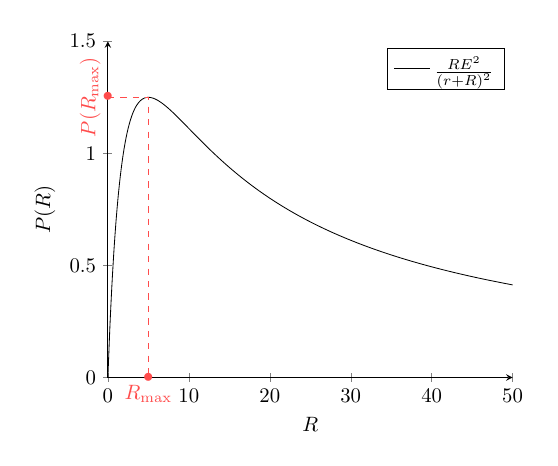
\begin{tikzpicture}[scale=0.75]
        \def\E{5}
        \def\r{5}
        \begin{axis}[
            axis lines=left,
            xmin=0, xmax=50,
            ymin=0, ymax=1.5,
            xlabel=$R$, ylabel=$P(R)$,
            clip=false]
            \addplot[
                domain=0:50,
                samples=200,
                smooth]
                {x*\E^2/(\r+x)^2};
                \addlegendentry{$\frac{RE^2}{(r+R)^2}$}
            \draw[dashed, Red!70]
            (0,1.25) node {$\bullet$} node [above, rotate=90]
            {$P(R_\mathrm{max})$} --++
            (5,0) --++
            (0,-1.25) node {$\bullet$} node[below] {$R_\mathrm{max}$};
        \end{axis}
    \end{tikzpicture}
    \tcblower
    \tcbsubtitle[before skip=\baselineskip,
    colback = darkgray!50!black,
    colframe = darkgray!50!black]{Calcul}
    Soit
    \begin{itemize}
        \item $ \left\{\begin{array}{rcl}
                    \textcolor{orange}{v}~: \Rb^+ & \rightarrow & \Rb^+\\
                    R                             & \mapsto     & \DS \textcolor{orange}{R}\\
            \end{array}\right.\quad\hspace{0.7em}\Longrightarrow
            \left\{\begin{array}{rcl}
                    \textcolor{Red}{v'}~: \Rb^+ & \rightarrow & \Rb^+\\
                    R                           & \mapsto     & \DS \textcolor{Red}{1}\\
            \end{array}\right.$
        \item $ \left\{\begin{array}{rcl}
                    \textcolor{Purple}{u}~: \Rb^+ & \rightarrow & \Rb^+\\
                    R                             & \mapsto     & \DS \textcolor{Purple}{r+R}\\
            \end{array}\right.\hspace{0.5em}\Longrightarrow
            \left\{\begin{array}{rcl}
                    \textcolor{brandeisblue}{u'}~: \Rb^+ & \rightarrow & \Rb^+\\
                    R                                    & \mapsto     & \DS \textcolor{brandeisblue}{1}\\
            \end{array}\right.$
    \end{itemize}
    Ainsi \bigbreak

        $ \left\{\begin{array}{rcl}
                    \textcolor{Purple}{u}^{\textcolor{ForestGreen}{{-2}}}~: \Rb^+ & \rightarrow & \Rb^+\\
                    R              & \mapsto     &
                    \frac{\textcolor{ForestGreen}{1}}{\textcolor{Purple}{(r+R)}^{\textcolor{ForestGreen}{2}}}\\
            \end{array}\right.\Rightarrow
            \left\{\begin{array}{rcl}
                    D[\textcolor{Purple}{u}^{\textcolor{ForestGreen}{{-2}}}]~: \Rb^+ & \rightarrow & \Rb^-\\
                    R                 & \mapsto     &
                    \frac{\textcolor{ForestGreen}{-2}\times\textcolor{brandeisblue}{1}}
                    {\textcolor{Purple}{(r+R)}^{\textcolor{Goldenrod}{3}}}\\
            \end{array}\right.$
    \bigbreak
    Et donc,
    \begin{align*}
        P'(R) & = \frac{\textcolor{ForestGreen}{-2}}
        {\textcolor{Purple}{(r+R)}^{\textcolor{Goldenrod}{3}}}
        \times \textcolor{orange}{R} + \textcolor{Red}{1}\times
        \frac{\textcolor{ForestGreen}{1}}
        {\textcolor{Purple}{(r+R)}^{\textcolor{ForestGreen}{2}}}\\
        P'(R) & = \frac{-2R}{(r+R)^3} + \frac{r+R}{(r+R)^3}
    \end{align*}
    Ainsi
    \begin{equation*}
        \boxed{P'(R) = \frac{r-R}{(r+R)^3}}
    \end{equation*}
    Et donc
    \begin{equation*}
        P'(R_\mathrm{max}) = 0 \Longrightarrow
        \textcolor{Red!70}{\boxed{R_\mathrm{max} = r}}
    \end{equation*}
    Avec
    \begin{equation*}
        \textcolor{Red!70}{\boxed{P(R_\mathrm{max}) = \frac{E^2}{4r}}}
    \end{equation*}
\end{NCexem}

\section{Résistances équivalentes}
\subsection{}
\begin{tcbraster}[raster columns=2, raster equal height=rows]
    \begin{NCprop}{Résultat attendu}
        \begin{center}
            \includegraphics{2parrequiv}
        \end{center}
    \end{NCprop}
    \begin{NCrapp}{Outil}
        L'association en parallèle de deux résistances $R_1$ et $R_2$ donne une
        résistance équivalente $ R_{\rm eq}$ telle que~:
        \begin{empheq}[box=\fbox]{equation*}
            \frac{1}{ R_{\rm eq}} = \frac{1}{R_1} + \frac{1}{R_2}
        \end{empheq}
    \end{NCrapp}
    \begin{NCimpo}{Attention !}
        Faites particulièrement attention à bien écrire $\DS \frac{1}{ R_{\rm
        eq}}$ et non pas simplement $ R_{\rm eq}$, même après 5 lignes de calcul
        quand c'est nécessaire. Pensez toujours à vérifier l'homogénéité d'un
        résultat littéral avant de l'encadrer. Cette erreur est une des plus
        communes.
    \end{NCimpo}
    \begin{NCexem}{Application}
        En mettant les deux termes sur même dénominateur~:
        \begin{align*}
            \frac{1}{ R_{\rm eq}} & = \frac{1}{R_1}\times \textcolor{orange}{
            \frac{R_2}{R_2}} + \frac{1}{R_2}\times \textcolor{orange}{
        \frac{R_1}{R_1}} \\
         \Leftrightarrow \frac{1}{ R_{\rm eq}} & = \frac{R_2 + R_1}{R_1R_2}\\
         \Leftrightarrow R_{\rm eq}            & = \frac{R_1R_2}{R_1+R_2}
        \end{align*}
    \end{NCexem}
\end{tcbraster}

\subsection{}
\begin{center}
    \begin{NCexem}[width=.5\linewidth]{Application}
        \[R_1 = R_2 = R \Longrightarrow \boxed{ R_{\rm eq} = \frac{R}{2}}\]
    \end{NCexem}
\end{center}

\subsection{}
\begin{tcbraster}[raster columns=2, raster equal height=rows]
    \begin{NCprop}{Résultat attendu}
        \begin{center}
            \includegraphics{3parrequiv}
        \end{center}
    \end{NCprop}
    \begin{NCrapp}{Outil}
        L'association en parallèle de trois résistances $R_1$, $R_2$ et $R_3$
        donne une résistance équivalente $ R_{\rm eq}$ telle que~:
        \begin{empheq}[box=\fbox]{equation*}
            \frac{1}{ R_{\rm eq}} = \frac{1}{R_1} + \frac{1}{R_2} + \frac{1}{R_3}
        \end{empheq}
    \end{NCrapp}
\end{tcbraster}
\begin{center}
    \begin{NCexem}[width=.5\linewidth]{Application}
        De la même manière que précédemment, la mise sous même dénominateur
        donne~:
        \begin{align*}
            \frac{1}{ R_{\rm eq}} & = \frac{R_2R_3}{R_1R_2R_3} +
            \frac{R_1R_3}{R_1R_2R_3} + \frac{R_1R_2}{R_1R_2R_3}\\
            \Leftrightarrow R_{\rm eq} & = \frac{R_1R_2R_3}{R_1R_2 + R_2R_3 +
            R_1R_3}
        \end{align*}
        qui est bien homogène à une résistance étant de la forme $\DS
        \frac{R^{\cancel{3}}}{\cancel{R^2}} = R$.
    \end{NCexem}
\end{center}

\subsection{}
\begin{center}
    \begin{NCexem}[width=.7\linewidth]{Application}
        \[R_1 = R_2 = R_3 = R \Longrightarrow R_{\rm eq} = \frac{R^3}{3R^2}
        \Leftrightarrow \boxed{R_{\rm eq} = \frac{R}{3}}\]
    \end{NCexem}
\end{center}

\subsection{}
\begin{tcbraster}[raster columns=2, raster equal height=rows]
    \begin{NCprop}{Résultat attendu}
        \begin{center}
            \includegraphics{nparrequiv}
        \end{center}
    \end{NCprop}
    \begin{NCexem}{Application}
        Il n'y a toujours qu'une seule formule attendue, et elle s'écrit~:
        \[ \frac{1}{R_{\rm eq}} = \underbrace{ \frac{1}{R} + \frac{1}{R} +
            \cdots + \frac{1}{R}}_{\textit{n fois}} \Leftrightarrow
        \boxed{R_{\rm eq} = \frac{R}{n}} \]
    \end{NCexem}
\end{tcbraster}

\section{Association de générateurs}

\begin{tcbraster}[raster columns=5, raster equal height=rows]
    \begin{NCdefi}[raster multicolumn=2]{Schéma}
        \subsection{}\vspace*{-20pt}
        \begin{center}
            \includegraphics{assogen_ser}
        \end{center}
    \end{NCdefi}
    \begin{NCrapp}[raster multicolumn=3]{Outil}
        %\vspace{-12pt}
        \subsection{}
        \textbf{Loi des mailles}~: la somme algébrique des tensions d'une maille
        est nulle (cf. exercice \ref{ch2:ex1}). Pour l'appliquer, on se donne un
        sens de lecture d'une maille, ici dans le sens direct mais peu importe,
        puis on peut~:
        \begin{itemize}
            \item Écrire les tensions traversées dans le même sens que leur
                flèche d'un côté du signe égal, les autres de l'autre côté~;
            \item Écrire les tensions traversées dans le même sens avec un «~+~»
                et les autres avec un «~-~», le tout devant «~$=0$~».
        \end{itemize}
    \end{NCrapp}
\end{tcbraster}
\begin{tcbraster}[raster columns=9, raster equal height=rows]
    \begin{NCexem}[raster multicolumn=4]{Application}
        Étant donné qu'il n'y a qu'une maille, il ne peut y avoir qu'une seule
        intensité dans le circuit. On pose donc $i_1 = i_2 = i$, et en applicant
        la loi des mailles on a
        \begin{align*}
            & U_{R_3} + U_{r_2} - E_2 + U_{r_1} - E_1 =
                0\\
            & \Leftrightarrow R_3i + r_2i + r_1i =
                E_1 + E_2\\
            & \Leftrightarrow i \left( r_1+r_2+R_3 \right) =
                E_1 + E_2\\
            & \Leftrightarrow \boxed{i = \frac{E_1 + E_2}{r_1+r_2+R_3}}
        \end{align*}
    \end{NCexem}    
    \begin{NCimpl}[raster multicolumn=5]{Schéma simplifié}
        \subsection{}
        L'expression que l'on a trouvée est en tout point similaire à celle du
        premier exercice si on considère qu'on a un générateur de force
        électromagnétique $E = E_1 + E_2$ et de résistance interne $r = r_1 +
        r_2$~; on peut donc dessiner~:
        \begin{center}
            \includegraphics{assogen_ser-simple}
        \end{center}
    \end{NCimpl}
\end{tcbraster}
\begin{tcbraster}[raster columns=2, raster equal height=rows]
    \begin{NCcoro}{Situation particulière}
        \subsection{}
        Quand $r_1$ et $r_2$ sont nulles, on se retrouve avec un générateur de
        résistance interne $r = 0$~: c'est donc un \underline{générateur idéal}.
    \end{NCcoro}
    \begin{NCimpo}{Conclusion}
        L'étude théorique précédente ne présente aucune incohérence ou
        impossibilité de pratique peu importe la situation, si tant est que les
        générateurs sont branchés dans le même sens~; si ça n'est pas le cas
        l'un considère l'autre comme un récepteur et le fait surchauffer.
    \end{NCimpo}
\end{tcbraster}

\begin{tcbraster}[raster columns=5, raster equal height=rows]
    \begin{NCdefi}[raster multicolumn=2]{Schéma}
        \subsection{}
        \vspace*{-12pt}
        \begin{center}
            \includegraphics{assogen_parr}
        \end{center}
    \end{NCdefi}
    \begin{NCexem}[raster multicolumn=3]{Générateurs idéaux}
        \subsection{}\vspace*{-20pt}
        \begin{center}
            \includegraphics{assogen_parr-ideal}
        \end{center}
        On doit trouver (avec l'unicité de la tension entre deux points, ici par
        exemple A et B) que $U_{R_4} = E_2 = E_1$.
    \end{NCexem}
\end{tcbraster}
\begin{center}
    \begin{NCprop}[width=.7\linewidth]{Conclusion}
        On ne peut brancher des générateurs idéaux de tension en parallèle que
        si leurs tensions sont les mêmes~; les générateurs réels peuvent l'être
        et ce sont les intensités qui vont s'adapter pour suivre la loi des
        mailles.
    \end{NCprop}
\end{center}

\section{Calculs de résistances équivalentes}

\subsection{Schéma 1}
\begin{center}
    \includegraphics{requiv_a}
\end{center}
La suite de schémas équivalents précédents donne~:
\begin{align*}
    R_{\rm eq}                 & = \textcolor{orange}{R + R} +
        \textcolor{brandeisblue}{R_{\rm eq,2}} \\
    \Leftrightarrow R_{\rm eq} & = \textcolor{orange}{2R} +
        \textcolor{brandeisblue}{\frac{
                R\times \textcolor{ForestGreen}{R_{\rm eq,1}}
        }{R + \textcolor{ForestGreen}{R_{\rm eq,1}}}}\\
    \Leftrightarrow R_{\rm eq} & = 2R + \frac{
        R\times\textcolor{ForestGreen}{2R}}{
        R+\textcolor{ForestGreen}{2R}} \\
    \Leftrightarrow R_{\rm eq} & = 2R + \frac{2R^{\cancel{2}}}{3\cancel{R}}\\
    \Leftrightarrow R_{\rm eq} & = \frac{8R}{3}
\end{align*}

\subsection{}
\begin{center}
    \includegraphics{requiv_b}
\end{center}
Et cette fois~:
\begin{align*}
    R_{\rm eq}                 & =
    \textcolor{orange}{R_1} + \color{brandeisblue}R_{\rm eq,2} \\
    \Leftrightarrow R_{\rm eq} & =
        R_1 + \textcolor{brandeisblue}{\frac{
        R_2\times \textcolor{ForestGreen}{R_{\rm eq,1}}}{
        R_2 + \textcolor{ForestGreen}{R_{\rm eq,1}}}} \\
    \Leftrightarrow R_{\rm eq} & =
        R_1 + \frac{R_2\times(r+R+R_2)}{r+R+2R_2}\\
\end{align*}

\subsection{}
Ce schéma est un peu plus compliqué, mais la bonne pratique de nommer des points
de potentiel sur un schéma aide à ne pas se perdre. En effet, étant donné que
l'on nous demande de déterminer la résistance équivalente entre A et B, toute
simplification du circuit est à faire. On a travaillé sur les associations de
résistances mais il ne faut pas oublier, et donc savoir reconnaître, les
potentiels court-circuits. Ici, en reportant le point A sur chaque point
d'intérêt où il peut être reporté (c'est-à-dire s'il n'y a pas de dipôle entre
les deux), on voit qu'un courant qui partirait de A pour aller à B (ce que fait
un Ohmmètre) éviterait complètement les trois premières résistances. On peut
redessiner le schéma différemment pour faire apparaître le court-circuit de
manière plus explicite~:

\begin{center}
    \includegraphics{requiv_c}
\end{center}

Ainsi, le circuit se simplifie en~:
\begin{center}
    \includegraphics{2parrequiv}
\end{center}
Soit
\[ \boxed{R_{\rm eq} = \frac{R_1R_2}{R_1 + R_2}}\]

\section{Conventions}
\subsection{Tout récepteur}
\begin{tcbraster}[raster columns=7, raster equal height=rows]
    \begin{NCdefi}[raster multicolumn=2]{Schéma}
        \subsubsection{}
        \vfill
        \begin{center}
            \includegraphics{convs_a}
        \end{center}
        \vfill
    \end{NCdefi}
    \begin{NCrapp}[raster multicolumn=2]{Calcul}
        \subsubsection{}
        \vfill
        \begin{itemize}[leftmargin=20pt]
            \item $P_{\text{r}}(E) = -EI$
            \item $P_{\text{r}}(r) = rI^2$
            \item $P_{\text{r}}(R) = RI^2$
        \end{itemize}
        \vfill
    \end{NCrapp}
    \begin{NCexem}[raster multicolumn=3]{Application}
        \subsubsection{}
        On a $\sum P_{\text{f}} = \sum P_{\text{r}}$, donc d'après
        la question précédente~:
        \begin{align*}
            0         & = -EI + rI^2 + RI^2\\
            I(r+R)    & = E\\
            \Aboxed{I & = \frac{E}{r+R}}
        \end{align*}
    \end{NCexem}
\end{tcbraster}

\subsection{Tout générateur}
\begin{tcbraster}[raster columns=7, raster equal height=rows]
    \begin{NCdefi}[raster multicolumn=2]{Schéma}
        \subsubsection{}
        \vfill
        \begin{center}
            \includegraphics{convs_b}
        \end{center}
        \vfill
    \end{NCdefi}
    \begin{NCrapp}[raster multicolumn=2]{Calcul}
        \subsubsection{}
        \vfill
        \begin{itemize}[leftmargin=20pt]
            \item $P_{\text{f}}(E) = EI$
            \item $P_{\text{f}}(r) = -rI^2$
            \item $P_{\text{f}}(R) = -RI^2$
        \end{itemize}
        \vfill
    \end{NCrapp}
    \begin{NCexem}[raster multicolumn=3]{Application}
        \subsubsection{}
        On a $\sum P_{\text{f}} = \sum P_{\text{r}}$, donc d'après
        la question précédente~:
        \begin{align*}
            EI - rI^2 - RI^2 & = 0\\
            I(r+R)           & = E\\
            \Aboxed{I        & = \frac{E}{r+R}}
        \end{align*}
    \end{NCexem}
\end{tcbraster}

\subsection{Conventions combinées}
\begin{tcbraster}[raster columns=7, raster equal height=rows]
    \begin{NCdefi}[raster multicolumn=2]{Schéma}
        \subsubsection{}
        \vfill
        \begin{center}
            \includegraphics{convs_c}
        \end{center}
        \vfill
    \end{NCdefi}
    \begin{NCrapp}[raster multicolumn=2]{Calcul}
        \subsubsection{}
        \vfill
        \begin{itemize}[leftmargin=20pt]
            \item $P_{\text{f}}(E) = EI$
            \item $P_{\text{r}}(r) = rI^2$
            \item $P_{\text{r}}(R) = RI^2$
        \end{itemize}
        \vfill
    \end{NCrapp}
    \begin{NCexem}[raster multicolumn=3]{Application}
        \subsubsection{}
        On a $\sum P_{\text{f}} = \sum P_{\text{r}}$~: avec les
        conventions adaptées, on a~:
        \begin{align*}
            EI        & = rI^2 + RI^2\\
            I(r+R)    & = E\\
            \Aboxed{I & = \frac{E}{r+R}}
        \end{align*}
    \end{NCexem}
\end{tcbraster}
\begin{center}
    \begin{NCcexe}[width=\linewidth]{Conclusion}
        On trouve bien toujours la même valeur de l'intensité dans le circuit,
        ce qui montre bien que les conventions ne sont que des conventions et ne
        changent pas la manière dont la physique fonctionne ensuite. Il faut
        noter cependant que le $I$ du premier schéma n'est pas le $I$ des
        schémas 2 et 3, étant donné que le sens n'est pas le même~: les
        intensitées sont opposées.
    \end{NCcexe}
\end{center}

\section{Mesures de tensions et intensités}
\begin{tcbraster}[raster columns=2, raster equal height=rows]
    \begin{NCrapp}{Rappel}
        \begin{center}
            \includegraphics{amp_parfait}
            \smallbreak
            \includegraphics{volt_parfait}
        \end{center}
    \end{NCrapp}
    \begin{NCdefi}[sidebyside]{Données}
        \begin{itemize}
            \item $E   = \SI{5.0}{V}$
            \item $r_1 = \SI{10}{\ohm}$
            \item $R   = \SI{20}{\ohm}$
        \end{itemize}
        \tcblower
        \begin{itemize}
            \item $R_1 = \SI{30}{\ohm}$
            \item $R_2 = \SI{40}{\ohm}$
        \end{itemize}
    \end{NCdefi}
\end{tcbraster}
\subsection{Schéma 1}
\begin{tcbraster}[raster columns=3, raster equal height=rows]
    \begin{NCdefi}{Schéma}
        \begin{center}
            \hspace*{-12pt}
            \includegraphics{mes_iu_a}
        \end{center}
    \end{NCdefi}
    \begin{NCimpl}{Simplification}
        \begin{center}
            \hspace*{-12pt}
            \includegraphics{mes_iu_a-simple}
        \end{center}
    \end{NCimpl}
    \begin{NCexem}{Application}

        V ouvre le circuit, donc aucun courant ne passe dans la boucle de
        droite~: A mesure \SI{0}{A}. On trouve $I$ avec la loi des mailles et on
        trouve $\DS I = \frac{E}{r_1 + R_1}$, et donc A' mesure \SI{0.125}{A}.
        Pour V, $R$ n'a pas de différence de potentiel donc il mesure $U_{R_1}
        = \SI{3.75}{V}$.

    \end{NCexem}
\end{tcbraster}
\subsection{Schéma 2}
\begin{tcbraster}[raster columns=2, raster equal height=rows]
    \begin{NCdefi}{Schéma}
        \begin{center}
            \includegraphics{mes_iu_b}
        \end{center}
    \end{NCdefi}
    \begin{NCimpl}{Simplification}
        \begin{center}
           \includegraphics{mes_iu_b-simple}
        \end{center} 
    \end{NCimpl}
\end{tcbraster}
\begin{center}
    \begin{NCexem}[width=.7\linewidth]{Application}
        Cette fois c'est la partie de droite qui est ouverte, et donc pas
        parcourue par un courant~: A mesure \SI{0}{V}. L'ampèremètre de gauche
        court-circuite quant à lui la résitance $R_2$, ainsi toute l'intensité
        se trouve dans la boucle où on a tracé \textcolor{brandeisblue}{$I$}~;
        une rapide loi des mailles donne $\DS I = \frac{E}{R} = \SI{0.25}{A}$. V
        ne mesure pas de différence de potentiel.
    \end{NCexem}
\end{center}

\section{Diviseur de tension}
\begin{tcbraster}[raster columns=3, raster equal height=rows]
    \begin{NCdefi}{Schéma}
        \begin{center}
            \includegraphics{divtens}
        \end{center}
    \end{NCdefi}
    \begin{tcolorbox}[blankest, raster multicolumn=1, space to=\myspace]
        \begin{tcbraster}[raster columns=1]
            \begin{NCprop}{Résultat attendu}
                On cherche $I$ puis $U_{BC}$.
            \end{NCprop}
            \begin{NCrapp}[add to natural height=\myspace]{Outils}
                \begin{itemize}[leftmargin=10pt]
                    \item Loi des mailles pour $I$~;
                    \item Loi d'Ohm pour $U_{BC}$.
                \end{itemize}
            \end{NCrapp}
        \end{tcbraster}
    \end{tcolorbox}
    \begin{NCexem}{Application}
        Il suffit d'une loi des mailles pour trouver
        \[I = \frac{E}{R_1+R_2}\]
        Puis trivialement
        \[U_{BC} = R_1I = \frac{R_1}{R_1+R_2}E\]
    \end{NCexem}
\end{tcbraster}
\begin{tcbraster}[raster columns=2, raster equal height=rows]
    \begin{NCrema}{Remarque}
        On remarque donc que deux dipôles de résistances $R_1$ et $R_2$ se
        partageant une tension totale $E$ vont se la répartir
        en respectant la fraction de résistance à laquelle chaque diôle
        participe. C'est également une simple moyenne pondérée.
    \end{NCrema}
    \begin{NCror}{Important}
        Ce résultat est bien plus général que pour deux dipôles et fonctionne
        avec $n$ dipôles \textbf{\textit{en série}} sur une branche. Il faut
        pouvoir se ramener à ce schéma précis pour appliquer la formule du pont
        diviseur de tension – que vous pouvez maintenant utiliser sans loi des
        mailles~: $\DS U_x = E\times \frac{R_x}{R_\mathrm{tot}}$
    \end{NCror}
\end{tcbraster}

\begin{tcbraster}[raster columns=3, raster equal height=rows]
    \begin{NCdefi}{Schéma}
        \begin{center}
            \includegraphics{divtens_b}
        \end{center}
    \end{NCdefi}
    \begin{tcolorbox}[blankest, raster multicolumn=1, space to=\myspace]
        \begin{tcbraster}[raster columns=1]
            \begin{NCexem}{Réponse}
                Oui, elle va changer puisqu'on a branché un nouveau dipôle.
            \end{NCexem}
            \begin{NCprop}{Résultat attendu}
                On cherche $I$ et $U_{BC}$.
            \end{NCprop}
            \begin{NCrapp}[add to natural height=\myspace]{Outils}
                \begin{itemize}[leftmargin=10pt]
                    \item Loi des mailles pour $I$~;
                    \item Loi d'Ohm pour $U_{BC}$.
                \end{itemize}
            \end{NCrapp}
        \end{tcbraster}
    \end{tcolorbox}
    \begin{NCinte}{Schéma simplifié}
        \begin{center}
            \includegraphics{divtens_b-simple}
        \end{center}
    \end{NCinte}
\end{tcbraster}
\begin{center}
    \begin{NCexem}[sidebyside]{Application}
        On peut envisager ce calcul de deux manières~:
        \begin{itemize}

            \item D'une part, $U_{BC} = R_1 I_1$ et on pourrait déterminer $I_1$
                en fonction de $I$ avec une LdN, et pour ça avoir $I$ avec une
                LdM en calculant $R_{\rm eq}$ comme précédemment, et donc~:

            \item On voit immédiatement que $U_{BC} = R_{\rm eq}I$. Autant
                partir là-dessus.
        \end{itemize}
        \tcblower
        On obtient ainsi \[ R_{\rm eq} = \frac{R_1R_3}{R_1+R_3} \quad \text{et}
        \quad I = \frac{E}{R_2 + \frac{R_1R_3}{R_1+R_3}}\] d'où après calcul
        \[\boxed{U_{BC} = \frac{ER_1R_3}{R_2(R_1+R_3)+R_1R_3}}\]
        %\quad \text{ou}
        %\quad \boxed{U_{BC} = \frac{E}{\frac{R_2}{R_3} + \frac{R_2}{R_1} + 1}}\]
    \end{NCexem}
\end{center}

\section{Diviseur de courant}
\begin{tcbraster}[raster columns=3, raster equal height=rows]
    \begin{NCdefi}{Schéma}
        \begin{center}
            \includegraphics{divcour}
        \end{center}
    \end{NCdefi}
    \begin{tcolorbox}[blankest, raster multicolumn=1, space to=\myspace]
        \begin{tcbraster}[raster columns=1]
            \begin{NCprop}{Résultat attendu}
                On cherche $U_{R_1}$ et $U_{R_2}$.
            \end{NCprop}
            \begin{NCrapp}[add to natural height=\myspace]{Outils}
                \begin{itemize}
                    \item Unicité de la tension en parallèle~;
                    \item Expression résistance $\parr$.
                \end{itemize}
            \end{NCrapp}
        \end{tcbraster}
    \end{tcolorbox}
    \begin{NCinte}{Schéma simplifié}
        \begin{center}
            \includegraphics{divcour-simple}
        \end{center}
    \end{NCinte}
\end{tcbraster}
\begin{tcbraster}[raster columns=2, raster equal height=rows]
    \begin{NCexem}{Application}
        On a certes $U_{R_1} = I_1R_1$ et $U_{R_2} = I_2R_2$, mais comme on a
        $U_{R_1} = U_{R_2} = U_{AB}$, le plus simple est de déterminer $U_{AB}$.
        Une résistance équivalente $R_{\rm eq} = \frac{R_1R_2}{R_1+R_2}$ avec
        l'intensité $I$ qui est connue (car imposée par le générateur de
        courant) donne facilement \[U_{R_1} = U_{R_2} = R_{\rm eq}I =
        \frac{R_1R_2}{R_1+R_2}I\]
    \end{NCexem}
    \begin{NCror}{Important}
        Ce résultat est la base de la réflexion menant à l'expression du
        diviseur de courant qui donne l'expression de $I_x$~: on voit
        directement apparaître que $\DS I_x = I\times\frac{R_{\rm eq}}{R_x}$ de par
        l'unicité de la tension. Souvenez-vous de cette simplicité.
    \end{NCror}
\end{tcbraster}

\begin{tcbraster}[raster columns=3, raster equal height=rows]
    \begin{NCprop}{Résultat attendu}
        On cherche $I_2$ en fonction de $I, R_1, R_2$ \textbf{à partir de la loi
        des mailles}.
    \end{NCprop}
    \begin{NCrapp}{Outils}
        -- LdM~: $I_1R_1 = I_2R_2 \quad \color{ForestGreen}(1)$~;
        \smallbreak
        -- LdN~: $I = I_1 + I_2 \quad \color{ForestGreen}(2)$.
    \end{NCrapp}
    \begin{NCexem}{Application}
        En utilisant \textcolor{ForestGreen}{(2)} dans
        \textcolor{ForestGreen}{(1)}, on a $I_2R_2 = (I-I_2)R_1$, donc en
        isolant $I_2$ on obtient facilement \[\boxed{I_2 = I
        \frac{R_1}{R_1+R_2}}\]
    \end{NCexem}
\end{tcbraster}
\begin{tcbraster}[raster columns=7, raster equal height=rows]
    \begin{tcolorbox}[blankest, raster multicolumn=4, space to=\myspace]
        \begin{tcbraster}[raster columns=1]
    \begin{NCdefi}{Schéma}
        \begin{center}
            \includegraphics{divcour_3}
        \end{center}
    \end{NCdefi}
    \begin{NCprop}{Résultat attendu}
        Évidemment, $I_2$ va changer puisqu'on branche un nouveau dipôle en
        parallèle. Une rivière qui se divise en 3 plutôt qu'en 2 va avoir des
        débits différents dans les deux situations. Donc on cherche $I_2$ en
        fonction de $I, R_1, R_2, R_3$ \textbf{sans méthode imposée}.
    \end{NCprop}
        \end{tcbraster}
    \end{tcolorbox}
    \begin{NCexem}[raster multicolumn=3]{Application}
        Avec la réflexion de la question 1 ou la relation du pont diviseur de
        courant qui est maintenant utilisable à volonté, on a facilement $I_2 =
        I\times \frac{R_{\rm eq}}{R_2}$. Avec $R_{\rm eq} =
        \frac{R_1R_2R_3}{R_1R_2+R_1R_3+R_2R_3}$, on a finalement
        \[\boxed{I_2 = I \times \frac{R_1R_3}{R_1R_2+R_1R_3+R_2R_3}}\]
    \end{NCexem}
\end{tcbraster}
\begin{tcbraster}[raster columns=2, raster equal height=rows]
    \begin{NCrema}{Remarque}
        L'intensité $I$ ne va pas changer, puisque c'est celle que l'on fixe
        avec le générateur.
    \end{NCrema}
    \begin{NCror}{Important}
        Bien que la loi des mailles soit l'origine de nombreuses relations, ici
        c'est la simple unicité de la tension qui amène au diviseur de courant.
    \end{NCror}
\end{tcbraster}

\section{Calcul d'intensité}
\begin{tcbraster}[raster columns=5, raster equal height=rows]
    \begin{NCdefi}[raster multicolumn=3]{Schéma}
        \subsection{}
        \begin{center}
            \includegraphics{calc_intens}
        \end{center}
    \end{NCdefi}
    \begin{tcolorbox}[blankest, raster multicolumn=2, space to=\myspace]
        \begin{tcbraster}[raster columns=1]
            \begin{NCprop}[add to natural height=\myspace]{Résultat attendu}
                On cherche à exprimer $I_2$.
            \end{NCprop}
            \begin{NCrapp}{{LdN, LdM}}
                \begin{itemize}
                    \item $I = I_1 + I_2 \color{ForestGreen}(1)$ (LdN)~;
                    \item $I_1R_1 + Ir_1 = E_1 \color{ForestGreen}(2)$ (LdM 1)~;
                    \item $I_2(R+R_2) = I_1R_1 \color{ForestGreen}(3)$ (LdM 2).
                \end{itemize}
            \end{NCrapp}
        \end{tcbraster}
    \end{tcolorbox}
\end{tcbraster}
\begin{tcbraster}[raster columns=2, raster equal height=rows]
    \begin{NCimpo}{Conseil}
        Pour les systèmes, il faut~: numéroter les équations qu'on veut
        réutiliser en premier lieu, à l'aide des $\color{ForestGreen}(1)$ par
        exemple, savoir qu'un système de 3 équations (indépendantes) à 3
        inconnues \underline{est} résolvable ensuite, et comprendre comment s'y
        prendre enfin. Cette dernière partie est bien sûr la vraie étape
        difficile et passe par la pratique, mais elle s'apprend.
    \end{NCimpo}
    \begin{NCrema}{Exemple}
        $I_2$ apparaît dans l'équation $\color{ForestGreen}(3)$, mais s'exprime
        en fonction de $I_1$ inconnu. On doit donc commencer par trouver une
        expression de $I_1$ utile. $I_1$ fait partie de l'équation
        $\color{ForestGreen}(2)$ qui, elle, dépend de $I$ mais en utilisant
        $\color{ForestGreen}(1)$ on peut facilement changer
        $\color{ForestGreen}(2)$ en une nouvelle équation reliant $I_1$ à $I_2$
        \underline{et qui n'est pas $\color{ForestGreen}(3)$} et qu'on
        appellera brillamment $\color{ForestGreen}(4)$. Ainsi, en réinjectant
        \textcolor{ForestGreen}{(4)} dans \textcolor{ForestGreen}{(3)}, on aura
        une expression de $I_2$ en fonction uniquement des paramètres du circuit
        ($E, R$).
    \end{NCrema}
\end{tcbraster}

\begin{center}
    \begin{NCexem}[sidebyside, righthand ratio=.55]{Application}
        Injecter \textcolor{ForestGreen}{(1)} dans \textcolor{ForestGreen}{(2)}
        donne~:
        \begin{align*}
            I_1R_1 + (I_1+I_2)r_1 &= E_1\\
            I_1(R_1+r_1) &= E_1-I_2r_1\\
            I_1 &= \frac{E_1 - I_2r_1}{R_1 + r_1} \quad \color{ForestGreen}(4)
        \end{align*}
        Ainsi, il suffit de réinjecter \textcolor{ForestGreen}{(4)} dans
        \textcolor{ForestGreen}{(3)} pour avoir~:
        \tcblower
        \begin{align*}
            I_2(R_2+R) &= \frac{E_1 - I_2r_1}{R_1 + r_1}\times R_1\\
            I_2(R_2+R)\times(R_1+r) &= (E_1-I_2r)\times R_1\\
            I_2 \left[ (R_2+R)(R_1+r_1)+r_1R_1 \right] &= E_1R_1
        \end{align*}
        et finalement
        \[\boxed{I_2 = \frac{E_1R_1}{\left[ (R_2+R)(R_1+r_1)+r_1R_1 \right]}}\]
    \end{NCexem}
\end{center}

\begin{tcbraster}[raster columns=2, raster equal height=rows]
    \begin{NCprop}[]{Résultat attendu}
        \subsection{}
        On cherche à trouver $I_2$ \textit{avec un diviseur de courant}.
    \end{NCprop}
    \begin{NCrapp}[sidebyside, righthand ratio=0.4]{Outil}
        \begin{center}
            \includegraphics[]{divcour}
        \end{center}
        \tcblower
        \begin{center}
            Dans le circuit ci-contre,
            \[ I_2 = \frac{R_{\rm eq}}{R_2}I\]
        \end{center}
    \end{NCrapp}
\end{tcbraster}
\begin{NCdefi}[]{Schéma}
    \includegraphics[width=\linewidth]{calc_intens-divcour}
\end{NCdefi}
\begin{NCexem}[breakable, sidebyside]{Application}
    Sur le schéma ci-dessus, on définit
    \[ \boxed{R_{\rm eq,1} = R+R_2} \qet \boxed{R_{\rm eq,2} =
        \frac{R_1(R+R_2)}{R + R_1 + R_2}}\]
    pour appliquer la relation du pont diviseur de courant~:
    \begin{equation*}
        I_2                 = \frac{R_{\rm eq, 2}}{R_{\rm eq,1}}I
        \Leftrightarrow I_2 = \frac{R_1}{R + R_1 + R_2}I
    \end{equation*}
    \tcblower
    Avec une loi des mailles on trouve
    \begin{equation*}
        I                 = \frac{E_1}{r_1 + R_{\rm eq,2}}
        \Leftrightarrow I = \frac{E_1}{r_1 + \frac{R_1(R+R_2)}{R + R_1 + R_2}}
    \end{equation*}
    Ainsi
    \begin{gather*}
        I_2 = \frac{R_1}{\cancel{\color{orange!70}R + R_1 + R_2}}
            \frac{E_1}{r_1 \textcolor{orange!70}{(R+R_1+R_2)}
                    + \frac{R_1(R+R_2)}{\cancel{\color{orange!70}R + R_1 +
                R_2}}}\\
        \Leftrightarrow \boxed{I_2 = \frac{R_1E_1}{(R+R_1+R_2)r_1 + R_1(R+R_2)}}
    \end{gather*}
    On trouve bien le même résultat (en développant un peu).
\end{NCexem}

\begin{tcbraster}[raster columns=2, raster equal height=rows]
    \begin{NCprop}[]{Résultat attendu}
        \subsection{}
        On cherche à trouver $I_2$ \textit{avec un diviseur de tension}.
    \end{NCprop}
    \begin{NCrapp}[sidebyside, righthand ratio=.4]{Outil}
        \begin{center}
            \includegraphics[width=\linewidth]{divtens-rangle}
        \end{center}
        \tcblower
        \begin{center}
            Dans le circuit ci-contre,
            \[ U_{R_2} = \frac{R_2}{R_1+R_2}E\]
        \end{center}
    \end{NCrapp}
\end{tcbraster}
\begin{NCexem}[breakable, sidebyside]{Application}
    Sur le schéma ci-dessus, on définit
    \[ \boxed{R_{\rm eq,1} = R+R_2} \qet \boxed{R_{\rm eq,2} =
        \frac{R_1(R+R_2)}{R + R_1 + R_2}}\]
    pour appliquer la relation du pont diviseur de tension~:
    \begin{equation*}
        I_2(R_{\rm eq,1}) = U_{AB} =
            \boxed{U_{R_{\rm eq,2}} = \frac{R_{\rm eq,2}}{r_1 + R_{\rm eq,2}}E}
    \end{equation*}
    \tcblower
    En développant on trouve
    \begin{gather*}
        I_2\cancel{(R+R_2)} =\\
            \frac{R_1\cancel{(R+R_2)}}{\cancel{\color{orange!70}R + R_1 + R_2}}
            \frac{E}{r_1 \textcolor{orange!70}{(R+R_1+R_2)}
                    + \frac{R_1(R+R_2)}{\cancel{\color{orange!70}R + R_1 +
                R_2}}}
    \end{gather*}
    Ce qui donne bien
    \begin{equation*}
        \boxed{I_2 = \frac{R_1E}{(R+R_1+R_2)r_1 + R_1(R+R_2)}}
    \end{equation*}
\end{NCexem}

\section{Association de générateurs~: application}
\begin{tcbraster}[raster columns=2, raster equal height=rows]
    \begin{NCdefi}{Schéma}
        \begin{center}
            \includegraphics{assogen_parr-ldm}
        \end{center}
    \end{NCdefi}
    \begin{tcolorbox}[blankest, space to=\myspace]
        \begin{tcbraster}[raster columns=1]
            \begin{NCprop}[add to natural height=\myspace]{Résultat attendu}
                On cherche $I_4$ puis $U_4 = R_4I_4$.
            \end{NCprop}
            \begin{NCrapp}{Outils}
                \begin{itemize}
                    \item LdM 1~: $I_4R_4 + I_1r_1 = E_1 \quad \color{ForestGreen}(1)$~;
                    \item LdM 2~: $I_4R_4 + I_2r_2 = E_2 \quad \color{ForestGreen}(2)$~;
                    \item LdN 1~: $I_1 + I_2 = I_4 \quad \color{ForestGreen}(3)$.
                \end{itemize}
            \end{NCrapp} 
        \end{tcbraster}
    \end{tcolorbox}
\end{tcbraster}
\begin{tcbraster}[raster columns=7, raster equal height=rows]
    \begin{NCror}[raster multicolumn=3]{Approche méthodique}
        Notre but est de trouver une équation contenant $I_4$ et des valeurs
        connues, c'est-à-dire tout sauf $I_1, I_2$.
        \bigbreak
        L'équation \textcolor{ForestGreen}{(1)} peut nous aider~; on peut la
        transformer en remplaçant $I_1$ par $I_4-I_2$ grâce à
        \textcolor{ForestGreen}{(3)} pour avoir une équation
        \textcolor{ForestGreen}{(4)} avec $I_4$ et $I_2$.
        \bigbreak
        Mais comme \textcolor{ForestGreen}{(2)} nous permet d'isoler $I_2$ et de
        l'exprimer en fonction de $I_4$, en injectant cette expression dans
        \textcolor{ForestGreen}{(4)} on obtient une équation entre $I_4$ et les
        éléments du circuit. Question résolue !
    \end{NCror}
    \begin{NCexem}[raster multicolumn=4]{Application}
        Avec \textcolor{ForestGreen}{(3)} dans \textcolor{ForestGreen}{(1)}~:
        \[I_4R_4 + (I_4-I_2)r_1 = E_1 \quad \color{ForestGreen}(4)\]
        En réexprimant \textcolor{ForestGreen}{(2)}~:
        \[I_2 = (E_2 - I_4R_4)/r_2\]
        En injectant \textcolor{ForestGreen}{(2)} dans
        \textcolor{ForestGreen}{(4)}~:
        \begin{align*}
            I_4(R_4+r_1) - (E_2-I_4R_4) \frac{r_1}{\color{brandeisblue}r_2}
                &= E_1\\
                \Leftrightarrow I_4(\textcolor{orange}{R_4} +
                                    \textcolor{red}{r_1})
                                    {\color{brandeisblue}r_2}
                                    -
                                    (E_2-I_4\textcolor{orange}{R_4})
                                    \textcolor{red}{r_1}
                &= E_1{\color{brandeisblue}r_2}\\
            \Leftrightarrow I_4(\textcolor{red}{r_1}
                                \textcolor{brandeisblue}{r_2} +
                                \textcolor{red}{r_1}\textcolor{orange}{R_4} +
                                \textcolor{brandeisblue}{r_2}\textcolor{orange}{R_4})
                &= E_1r_2 +E_2r_1
        \end{align*}
        Soit
        \[\boxed{I_4 = \frac{E_1r_2 + E_2r_1}{r_1r_2+r_1R_4+r_2R_4}} \quad
        \text{et} \quad \boxed{U_{R_4} = R_4\times I_4}\]
    \end{NCexem}
\end{tcbraster}

\section{Pont de Wheatstone}

\begin{tcbraster}[raster columns=6, raster equal height=rows]
    \begin{NCdefi}[raster multicolumn=2]{Schéma}
        \begin{center}
            \includegraphics{wheatstone}
        \end{center}
    \end{NCdefi}
    \begin{tcolorbox}[blankest, raster multicolumn=1, space to=\myspace]
        \begin{tcbraster}[raster columns=1]
            \begin{NCprop}[add to natural height=\myspace]{Résultat attendu}

                \fontsize{10pt}{12pt}\selectfont On cherche $R_i$, ou $U_{DC}$
                quand «~le pont est équilibré~».

            \end{NCprop}
            \begin{NCrapp}{Outil}

                \fontsize{10pt}{12pt}\selectfont D'après l'énoncé, le pont est
                équilibré quand $V = 0$, soit quand $V_B = V_D$.

            \end{NCrapp}
        \end{tcbraster}
    \end{tcolorbox}
    \begin{NCexem}[raster multicolumn=3]{Application}
        Si le pont est équilibré, alors $U_{AB} = U_{AD}$ et $U_{BC} = U_{DC}$.
        Or, avec le pont diviseur de tension, on a à la fois
        \begin{align*}
            U_{BC} & = E \frac{R_1}{R_1+R}\\
            U_{DC} & = E \frac{R_i}{R_i+R_2}
        \end{align*}
        Donc
        \begin{align*}
            U_{BC} &= U_{DC}\\
            \Leftrightarrow \cancel{E} \frac{R_1}{R_1+R}
                   & = \cancel{E} \frac{R_i}{R_i+R_2}\\
            \Leftrightarrow R_1(\cancel{R_i}+R_2) & = R_i(\cancel{R_1}+R)\\
            \Leftrightarrow \Aboxed{R_i & = \frac{R_1R_2}{R}}
        \end{align*}
    \end{NCexem}
\end{tcbraster}

\section{Ponts diviseurs de tension}
\begin{center}
    \begin{NCrapp}[sidebyside, halign=center, halign lower=center,
        width=\linewidth]{Outil}
        \begin{center}
            \includegraphics[width=\linewidth]{divtens-rangle_3r}
        \end{center}
        \tcblower
        \begin{center}
            Dans le circuit ci-contre,
            \[\boxed{U_{R_x} = \frac{R_x}{R_{\rm eq}}E}\]
        \end{center}
    \end{NCrapp}
\end{center}

\begin{tcbraster}[raster columns=4, raster equal height=rows]
    \begin{NCdefi}[]{Schéma}
        \begin{center}
            \hspace*{-13pt}\includegraphics[width=1.2\linewidth]{pdt_a}
        \end{center}
    \end{NCdefi}
    \begin{NCexem}[]{Application}
        \subsection{}
        On a directement
        \[ \boxed{U_1 = - \frac{1}{3}E}\]
    \end{NCexem}
    \begin{NCdefi}[]{Schéma}
        \begin{center}
            \includegraphics[width=\linewidth]{pdt_b}
        \end{center}
    \end{NCdefi}
    \begin{NCexem}[]{Application}
        \subsection{}
        Avec la rotation du schéma, on voit facilement que
        \[ \boxed{U_2 = \frac{2}{3}E}\]
    \end{NCexem}
    \begin{NCdefi}[]{Schéma}
        \begin{center}
            \hspace*{-15pt}\includegraphics[width=1.2\linewidth]{pdt_c}
        \end{center}
    \end{NCdefi}
    \begin{NCexem}[]{Application}
        \subsection{}
        Ici, on remarque que $U_{AB} = E$. Ainsi
        \[ \boxed{U_3 = - \frac{2}{5}E}\]
    \end{NCexem}
    \begin{NCdefi}[]{Schéma}
        \begin{center}
            \includegraphics[width=\linewidth]{pdt_d}
        \end{center}
    \end{NCdefi}
    \begin{NCexem}[]{Application}
        \subsection{}
        $R_{\rm eq,1} =\DS \frac{2R^{\cancel{2}}}{3\cancel{R}} = \frac{2R}{3}$, d'où
        \[ \boxed{U_4 = \frac{3}{4}E}\]
    \end{NCexem}
\end{tcbraster}

\section{Pont diviseur de courant}

\begin{NCrapp}[sidebyside]{Outil}
    \begin{center}
        \includegraphics[]{divcour_3-eq}
    \end{center}
    \tcblower
    \begin{center}
        Dans le circuit ci-contre,
        \[ \boxed{I_x = \frac{R_{\rm eq}}{R_x}I}\]
    \end{center}
\end{NCrapp}
\begin{NCdefi}[]{Schéma}
    \begin{center}
        \includegraphics[width=\linewidth]{divcour_last-a}
    \end{center}
\end{NCdefi}
\begin{NCexem}[]{Application}
    En premier lieu,
    \[ I = \frac{\frac{2r}{3}}{r}I_d = \frac{2}{3}I_d\]
    Ensuite,
    \[ I_d = \frac{ \frac{2r}{5}}{ \frac{2r}{3}}I_0 = \frac{3}{5}I_0\]
    Ainsi,
    \[ \boxed{I = \frac{2}{5}I_0}\]
\end{NCexem}

\end{document}
